% !TEX root = mainthesis.tex
%Chapter 7

\renewcommand{\thechapter}{7}

\chapter{Topological order in quantum systems}
\label{ch:Topology}

Topological order can be found in a wide range of physical systems, from crystalline solids\cite{hasan_colloquium:_2010}, photonic meta-materials\cite{ozawa_topological_2019} and even atmospheric waves\cite{delplace_topological_2017} to optomechanic\cite{peano_topological_2015}, acoustic\cite{yang_topological_2015} and atomic systems\cite{cooper_topological_2019}. Topological systems are a robust foundation for creating quantized channels for transporting electrical current, light, and atmospheric disturbances. These topological effects can be quantified in terms of integer-valued invariants such as the Chern number, applicable to the quantum Hall effect\cite{thouless_quantized_1982,haldane_model_1988}, or the $\mathbb{Z}_2$ invariant suitable for topological insulators\cite{kane_$z_2$_2005}. 

We got interested in topology when working on engineering Rashba~\cite{bychkov_oscillatory_1984} type spin-orbit coupling in the lab. Our system has non-trivial topology but it breaks from the conventional mold used to describe topological materials. 

In this Chapter I take a step back to describe `conventional' topology before going into the unconventional. I will give a general overview of the basic concepts of topology in physics and its application to band theory of solids. The ideas of topology and how exactly one can connect donuts with band structures might feel quite obscure and complicated for non-experts in the field. I wrote this Chapter with that in mind, with the hope that it can be followed by non-experts and provide some insight and intuition about this field. The concepts introduced in this Chapter will be necessary for understanding the results presented in Chapter~\ref{ch:Rashba}.
 

\section{Topology in mathematics} 

Topology is a branch of mathematics that studies continuity. The most familiar example might be that of objects being continuously deformed into one another. For example, a donut can be continuously deformed into a coffee mug but if we want to deform it into a pretzel we need to poke more holes in it. This gives us some intuition that the donut and the mug must share the same topology, which is different from that of the pretzel. Topology also studies more abstract objects but I will limit the discussion to closed two-dimensional surfaces in three dimensions. This example will also be helpful to provide some intuition when we define topological invariants for band structures in the following sections.  

The topology of 2D surfaces can be classified by the Euler characteristic, and it is related to the local Gaussian curvature of the surface by the Gauss-Bonet theorem. The Gaussian curvature can be interpreted in the following way: at any point in a surface we can find a normal vector which which is orthogonal to the tangent plane of the surface. We can then define a family of planes containing the normal vector and their intersection with the surface defines a family of curves. The curvature of a given curve is called the normal curvature $\kappa$. When we consider all the normal curvatures, the minimum and maximum of these are called the principal curvatures and are used to define the Gaussian curvature at any point of a surface $K=\kappa_{min}\kappa_{max}$~\cite{differential_topology_and_geometry} 

The Gauss-Bonnet theorem states that the integral of the local Gaussian curvature over the whole surface is equal to the integer valued Euler characteristic
%
\begin{equation}
	\chi = \frac{1}{2\pi}\int_S K dA,
	\label{eq:euler_characteristic}
\end{equation}
%
which is related to the genus (number of holes or handles) by $\chi=2(1-g)$. The Gauss-Bonnet theorem is a very powerful result as it relates the local properties of a surface,the Gaussian curvature, with a global topological invariant, the Euler characteristic. 

In the following sections I will introduce topological invariants in the context of condensed matter physics, which even though might seem a bit more abstract, their interpretation can be closely related to the concepts just defined in this section.

\section{Topological order in condensed matter}

Just like topology classifies properties of geometric objects, one important task of condensed matter physics has been to classify phases of matter. Many of these phases, for example magnetic or conducting phases, can be described in terms of order parameters related to spontaneously broken symmetries~\cite{landau_theory_1936}. However, in the past few decades and increasing number of systems have been found where it is only possible to understand their phases and properties in terms of the underlying topology of their quantum states. This new paradigm of physics has been so important that in 2016 the Nobel prize in physics was awarded to David J. Thoules, F. Duncan M. Haldane and J. Michael Kosterlitz for the theoretical discoveries of topological phase transitions and topological phases of matter 

The effect of topology in condensed matter systems was first observed when von Klitzing and colleagues~\cite{klitzing_new_1980} measured quantized Hall resistance in two-dimensional electron gases subjected to a strong perpendicular magnetic field. The effect can be understood semi-classically by thinking of the electrons quantized cyclotron orbits that give rise to Landau levels. If the Landau levels are filled then there is an energy gap separating two consecutive levels and the material acts as an insulator but if an electric field is applied the orbits drift and the electrons will be `skipping orbits' in the edge, giving rise to what is known as edge states. 

In a seminal paper Thoules, Kohomoto, Nightingale, and den Nijs~\cite{thouless_quantized_1982} explained that the quantization of the Hall conductivity is determined by the underlying topology of the band structure. Just like the Euler characteristic defined in Equation~\ref{eq:euler_characteristic} classifies 2D solids that can be continuously deformed without opening or closing holes, there is a topological invariant that classifies band structures that can be deformed into one another without opening or closing an energy gap. This invariant, initially known as the `TKNN invariant', was later recognized by the mathematical physicist Bary Simon as the `first Chern class invariant from $U(1)$ fiber bundles'~\cite{simon_holonomy_1983}\footnote{See~\cite{geometry_topology_physics} for example if you want to learn more about this subject.} and the TKNN invariant became what is known today as the Chern number or Chern invariant. Another very valuable contribution from Simon's work was that he made the connection between the Chern number and the the Berry's geometrical phase~\cite{berry_michael_victor_quantal_1984} which will be defined in the following sections and will allow us to make a physical interpretation of this otherwise abstract seeming topological invariant. 

\section{Berry phase and Berry curvature}

A Berry or geometric phase is used to describe the phase acquired by a quantum state as it goes through a closed trajectory in parameter space. It plays a key role in topological band theory and can help to provide a physical interpretation of the Chern number. 

Consider a Hamiltonian $\hat H$ that depends on a set of parameters $\r=(r_1, r_2, ...)$. If the system parameters are slowly changed in time, the change in the system can be described by a path in parameter space $\r(t)$. The state $\ket{\psi(t)}$ evolves according to the time dependent Sch\"odinger equation and at any given time $t$ there is a basis that satisfies
%
\begin{equation}
	\hat H(\r)\ket{n(\r)}=E_n(\r)\ket{n(\r)}
	\label{eq:hamiltonian_eigenvectors}
\end{equation}
%
for $\r=\r(t)$. Suppose the system is initially in state $\ket{n(\r(t=0))}$, if the parameters are changed slowly such that the adiabatic theorem is valid then at time $t$ the state of the system can be written as
%
\begin{equation}
	\ket{\psi(t)}=\exp\Big\{-\frac{i}{\hbar}\int_0^tdt'E_n(\r(t'))\Big\}\exp(i\gamma_n(t))\ket{n(\r(t))},
	\label{eq:berry_wf}
\end{equation}
%
where the first term corresponds to a dynamical phase factor, and the second term is a geometric phase. A classical analogy to this geometric phase is that acquired by By imposing that $\ket{\psi(t)}$ satisfies the time-dependent Schr\"odinger equation one finds that 
%
\begin{equation}
	\gamma_n(t)=i\braket{n(\r)}{\nabla_{\r}n(\r)}\cdot\dot{\r}(t),
\end{equation}
%
where the term
%
\begin{equation}
	\mathbf{A}_n(\r)=i\braket{n(\r)}{\nabla_{\r}n(\r)}
	\label{eq:berry_connection}
\end{equation}
%
 is usually referred to as the Berry connection\footnote{This is reminiscent of the connection defined in differential geometry that is used to describe things like parallel transport.} or the Berry vector potential for reasons that will become apparent. Because eigenvectors can only be defined up to a global phase, $\mathbf{A}$ is a gauge dependent quantity. If we make a gauge transformation such that $\ket{n(\k)}\rightarrow\e^{i\xi(\k)}\ket{n(\k)}$ then the Berry connection is also transformed as $\mathbf{A}_n(\k)\rightarrow\mathbf{A}_n(\k)-\nabla_{\k}\xi(\k)$. However if we integrate the Berry connection on a closed loop
%
\begin{equation}
	\gamma_n(\mathcal{C})=\oint_{\mathcal{C}} \mathbf{A}_n(\r)\cdot d\mathbf{l},
	\label{eq:berry_phase}
\end{equation}
%
we obtain the Berry phase which is gauge independent (modulo $2\pi$).
and here it is important to note that $\gamma_n$ only depends on the geometry of the path and is independent of how it was traversed in time, and unlike the Berry connection, it is gauge independent quantity. 

An alternative way to compute Berry's phase uses Stoke's theorem from vector calculus
%
\begin{equation}
	\oint_{\mathcal{C}} \mathbf{A}_n\cdot d\mathbf{l}=\int_{\mathcal{S}}\nabla\times\mathbf{A}_n\cdot d\mathbf{S},
	\label{eq:berry_connection}
\end{equation}
%
where the vector field $\mathbf{\Omega}_n=\nabla\times\mathbf{A}_n$ is known as the Berry connection. 

Using the some vector calculus identities the Berry connection can be rewritten as

\begin{align}
	\mathbf{\Omega}_n=&i[\nabla_{\r}\bra{n}]\times[\nabla_{\r}\ket{n}]\nonumber \\ 
	=& \sum_{j\neq n} i[\bra{n}\nabla_{\r}\ket{j}]\times[\bra{j}\nabla_{\r}\ket{n}] \nonumber \\
	=& i\sum_{j\neq n}\frac{\bra{n}\nabla_{\r}\hat{H}\ket{j}\times\bra{j}\nabla_{\r}\hat{H}\ket{n}}{(E_j-E_n)^2},
	\label{eq:alternative_berry_con}
\end{align}
%
where $\bra{n}\nabla_{\r}\ket{j}$ was replaced with $\bra{n}\nabla_{\r}\hat{H}\ket{j}/(E_j-E_n)$ by differentiating Equation~\ref{eq:hamiltonian_eigenvectors}. This expression shows that $\mathbf{\Omega_n}$ is a gauge independent quantity as it does not depend on the derivatives of a particular gauge choice for $\ket{n}$ but rather on $\nabla_{\r}\hat{H}$ which is gauge independent. Also we can see that $\mathbf{\Omega}_n$ becomes singular when there are degeneracies present in the Hamiltonian. Degeneracies act as `sources' for the Berry connection and the Berry phase can be related to the number of singularities in $\mathbf{\Omega}_n$ enclosed by the adiabatic path. Finally, even though the system may remain in state $\ket{n}$ during the adiabatic evolution, this expression for the Berry curvature makes it explicit that other eigenstates of the Hamiltonian have an influence in the Berry phase acquired. 

\subsection{Aharonov-Bohm phase as an example of a Berry's phase}

A familiar example of geometric phases is the Aharonov-Bohm phase~\cite{aharonov_significance_1959} gained by an electrons making closed trajectories around a solenoid. This phase was initially conceived as way of showing that in quantum mechanics magnetic vector potentials, typically conceived only as mathematical objects, can have a physical effect on the wave function. They considered a coherent electron beam split into two paths around a solenoid that produces a magnetic field $\mathbf{B}$ as shown in Figure~\ref{fig:aharonov_bohm}. Outside the solenoid the magnetic field $\mathbf{B}=0$, but there can be a non-zero magnetic vector potential such that $\mathbf{B}=\nabla\times\mathbf{A}$. The two beams are later recombined. Even though the electron's trajectories are not modified, when looking at the interference pattern one finds that the two paths acquired different phases, and their difference is remarkably equal to magnetic flux across the area enclosed by the electrons path $\Delta\varphi = 2\pi \Phi_B/\Phi_0$, where $\Phi_0=h/e$ is the flux quantum. 

\begin{figure*}[htb]
\begin{center}
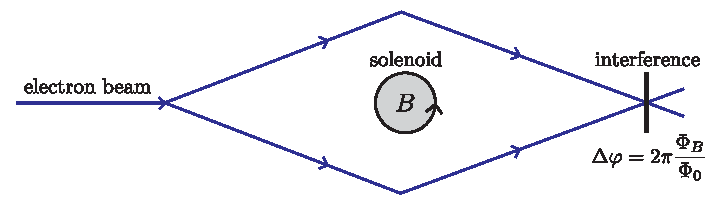
\includegraphics[]{Figures/Chapter7/aharonov_bohm.pdf}
\caption[The Aharonov-Bohm experiment]{The Aharonov-Bohm experiment. A coherent electron beam is split into two paths surrounding a solenoid which produces a non-zero magnetic field $\mathbf{B}$ inside the gray region and $\mathbf{B}=0$ outside. The two beams are later recombined and an interference pastern reveals a phase difference $\Delta\varphi = 2\pi \Phi_B/\Phi_0$ equal to the magnetic flux enclosed by the electron's path}
\label{fig:aharonov_bohm}
\end{center}
\end{figure*}

This Aharonov-Bohm phase can be interpreted as an example of a Berry phase in real space. For a charged particle in the presence of a vector potential the momentum dependence of the free-particle Hamiltonian is modified $\mathbf{p}\rightarrow\mathbf{p}-q\mathbf{A}$ so that the wave function will depend on the magnetic vector potential as well. Using Equations~\ref{eq:berry_connection} and~\ref{eq:berry_phase} it can be shown that the Berry phase associated to a closed path around the solenoid is exactly equal to the Aharonov-Bohm phase: 
%
\begin{align}
	\gamma_n(\mathcal{C})=&\frac{e}{\hbar}\oint_{\mathcal{C}}\mathbf{A}(\mathbf{r})\cdot d\mathbf{r} \nonumber \\
	=& \frac{e}{\hbar}\int_{\mathcal{S}}\nabla\times\mathbf{A}\cdot d\mathbf{S} \nonumber \\
	=& \frac{e\Phi_B}{\hbar},
	\label{eq:aharonov_bohm_phase}
\end{align}

For this particular example, the Berry connection is exactly equal to the magnetic vector potential and the Berry curvature is the magnetic field. This gives us a very physical intuition for interpreting the Berry phase in terms of the `magnetic flux' from abstract sources of `magnetic fields' in parameter space.  

\subsection{Chern number}

The Chern number is used to describe the topology of Bloch bands, where the relevant parameter space is defined by the crystal momentum in the Brillouin zone (BZ), which has the geometry of a torus due to the periodic boundary conditions. The Chern number of the $n$th band is defined as
%
\begin{equation}
	C_n=\frac{1}{2\pi}\int_{BZ}\mathbf{\Omega}_n d\k,
	\label{eq:chern_number}
\end{equation}
%
and is closely related to the definition of Berry phase from Equation~\ref{eq:berry_connection}. For our previous example of a quantum hall system, the integer in the quantized conductance is exactly equal to the Chern number. 

Just like two-dimensional surfaces are classified by the integral of their Gaussian curvature, the topology of Bloch bands and of quantum systems in general is determined by the integral of the Berry curvature. In a similar way, the integral connects local properties of a quantum system, the Berry connection, with a global topological invariant, the Chern number. One subtle difference is that the Euler characteristic is only determined by the surface (and its intrinsic Gaussian curvature) while the Chern number is defined both by a surface (the BZ) and an additional local curvature (the Berry curvature). By studying different Hamiltonians one can obtain a different Berry curvature, but the geometry of the BZ and thereby the surface of integration is defined by a torus\footnote{See next chapter for an example for when this breaks down.}. This difference will be important later on when we describe the experiments performed to study a system with Rashba spin-orbit coupling and an unconventional topology. %Using our intuition from the Aharonov-Bohm phase, the Chern number can also be interpreted as the total flux from a `Berry field'  defined in the BZ and whose sources are `monopoles' given by degeneracies in the Hamiltonian. 

% Even though the Chern invariant was initially conceived to classify the topology of systems in momentum space, there have been experiments that studied the topology of quantum systems in other abstract parameter spaces, see for example ~\cite{roushan_observation_2014} and \cite{sugawa_second_2018}.

\section{The bulk-edge correspondence principle}
\note{Debating if this should be a section...}

\section{Example: two-level model}

Many of the concepts introduced in the previous section can be readily applied and understood using a two-level model
%
\begin{equation}
	\hat{H}(\mathbf{k})= \mathbf{h}(\mathbf{k})\cdot\boldsymbol{\sigma}
	\label{eq:2D_Hamiltonian}
\end{equation}
%
where $\boldsymbol{\sigma}=(\sigma_x, \sigma_y, \sigma_z)$ are the Pauli matrices and $\mathbf{h}(\mathbf{k})=(h_x(\k),h_y(\k), h_z(\k))$. This model has been used to describe a number of physical systems like graphene~\cite{haldane_model_1988} and spin-orbit coupled systems~\cite{bychkov_oscillatory_1984,dresselhaus_spin-orbit_1955}. Lets now consider the simple case $h(\k)=\k$, for which $\nabla_{\k}\hat{H}=\boldsymbol{\sigma}$ and using Equation~\ref{eq:alternative_berry_con} it can be shown that
%
\begin{equation}
	\mathbf{\Omega}=\frac{\mathbf{h}}{h^3}
\end{equation}
%
which can be recognized as the field of a Dirac monopole~\cite{dirac_paul_adrien_maurice_quantised_1931}, which arises from the degeneracy between the two eigenstates at the origin. In the vicinity of the degeneracy the Hamiltonian can b(everything can be approximated by a line if you look close enough) It then follows that the Berry phase gained by moving in a closed path $\mathcal{C}$around the monopole is equal to the flux from the monopole in the surface enclosed by $\mathcal{C}$. This connects nicely with our intuition from the Aharonov-Bohm effect. 



\begin{figure*}[htb]
\begin{center}
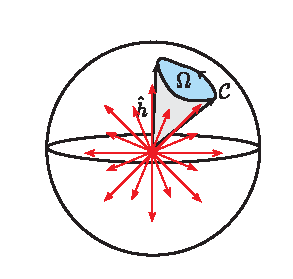
\includegraphics[]{Figures/Chapter7/solid_angle.pdf}
\caption{Stuff}
\label{fig:solid_angle}
\end{center}
\end{figure*}


% In particular, when C corresponds to a 2π rotation of dˆ in a plane, the Berry
% phase is π. The Berry curvature is given by the solid angle per unit area in k
% space, which is simply half the solid angle element for the mapping

% For this two-level system the Chern number can be written as
%
\begin{equation}
	C=\frac{1}{4\pi}\int(\partial_{k_x}\hat{h}\times\partial_{k_y}\hat{h})\cdot\hat{h} \, d\k
\end{equation}
%
which counts the number is equal to the number of times that the vector $\hat{h}(\k)=\mathbf{h}(\k)/\vert \mathbf{h}(\k)$ wraps around the Bloch sphere~\cite{kaufmann_notes_2016}, a quantity that is known as the winding number. %For a small and constant value of $h_z$, $\hat{h}$ only wraps around the top or lower half of the Bloch sphere, depending on the sign of $h_z$.

If $h_z=0$ there are Dirac points\footnote{This can happen if there is inversion ($\mathcal{P}$) and time reversal ($\mathcal{T}$) symmetry} where $\vert\mathbf{h}\vert=0$ and near these ponits Equation~\ref{eq:2D_Hamiltonian} locally resembles the Hamiltonian of a massless Dirac fermion. Near the Dirac points the Berry connection can be written as
%
\begin{equation}
	\mathbf{\Omega}=\frac{1}{2}\frac{\mathbf{h}}{h^3}
\end{equation}
%


\note{I am confused again... why is the Chern number not a quarter?}

Also keep in mind Krammers theorem: for every energy eigenstate of a time-reversal symmetric system with half-integer total spin, there is at least one more eigenstate with the same energy. In other words, every energy level is at least doubly degenerate if it has half-integer spin.

Why is $h_z\neq0$ the same as breaking time reversal symmetry? WHat about the other components? 
\section{Guauges and Dirac strings}

If magnetic monopoles exist then electric charge must be quantized
In electromagnetic theory 

A consequence of the Berry connection being singular 

This vector potential has one problem. It is singular at the north pole (z = r). In fact, one can prove that no matter which gauge one uses, there will always be a singularity point.

Degeneracies as sources of Berry curvature field. There must therefore be Dirac strings as well...


To finalize our introduction to Topology, Figure~\ref{fig:topology_analogies} summarizes all the concepts that have been introduced so far and is a reminder that topological invariants are global properties defined in terms of integrals of local properties and that we can use our intuition from electromagnetic theory to interpret Chern numbers. 

 \begin{figure*}[htb]
\begin{center}
\includegraphics[]{Figures/Chapter7/topology_analogies.pdf}
\caption[Different topological invariants]{The Euler characteristic and the Chern number are topological invariants defined by integrals of local curvatures. The Aharonov-Bohm phase gives us physical intuition to interpret the Chern number as the flux from a `Berry field'.}
\label{fig:topology_analogies}
\end{center}
\end{figure*}

%%%%%%%%%%%%%%%%%%%%%%%%%%%%%%%%%%%%%%%%%%%%%%%%%%%%%%%%%%%%%%%
%
%Graveyard
%
%%%%%%%%%%%%%%%%%%%%%%%%%%%%%%%%%%%%%%%%%%%%%%%%%%%%%%%%%%%%%%%%

% For this case the vector $\hat{h}(\k)$ is confined to the equator and does not wrap around the Bloch sphere. For small $h_z\neq0$ $\hat{h}(\k)$ covers  

% If there is inversion ($\mathcal{P}$) and time reversal ($\mathcal{T}$) symmetry $h_z(\k)=0$ and there are points where the Hamiltonian in Equation~\ref{eq:2D_Hamiltonian} becomes singular. For example, in graphene this occurs in two points. In the vicinity of these points $\q=\k-\k_0$, Equation~\ref{eq:2D_Hamiltonian} resembles the Hamiltonian of a massles Dirac fermion $\hat H(\mathbf k)=\hbar v_F\mathbf q\cdot \vec \sigma$, where $v_F$ is a velocity. 
 
% The $\mathcal{T}$ symmetry can be broken for example by applying a magnetic field, in which case the degeneracy at the Dirac point is broken and \ref{eq:2D_Hamiltonian} becomes a massive Dirac Hamiltonian. 


%  For simplicity lets consider $\mathbf{h}(\k)=h(\sin\theta\cos\phi,\sin\theta\sin\phi,\cos\theta)$. The Hamiltonian has eigenvalues $\pm h$ and the eigenstates are
% %
% \begin{align}
% 	\ket{+}=&(\sin\theta/2e^{-i\phi}, -\cos\theta/2 )  \nonumber \\
% 	\ket{-}=&(\cos\theta/2e^{-i\phi}, \sin\theta/2) 
% \end{align}
%

% \subsection{A physical interpretation of the Chern number}

% Consider a generic system that is described by the Hamiltonian

% \begin{equation}
% 	\hat H =\left(\frac{\hbar^2\mathbf{k}^2}{2m}+\hat{V}({\mathbf{r}})\right)\hat{\mathbb{1}} + \mathbf{\Omega}(\mathbf{r})\cdot\hat{\mathbf{F}}
% 	\label{eq:generic_topologic_Hamiltonian} 
% \end{equation}
% %
% where the vector $\mathbf{\Omega}(\mathbf r)=(\Omega_x(\r), \Omega_y(\r), \Omega_z(\r))$ describes a momentum dependent `magnetic field' or coupling between internal states and $\hat{\mathbf{F}}=(\fx, \fy, \fz)$. The eigenstates of~\ref{eq:generic_topologic_Hamiltonian} take the form
% %
% \begin{equation}
% 	\ket{\psi_n(\r)}=\sum_{i}a_{i,n}(\k)\ket{i,\Omega(\r)}
% 	\label{eq:generic_wavefunction}	
% \end{equation}



